\documentclass[a4paper,12pt]{article}
\usepackage{amsmath, amsthm, amssymb}
\usepackage{tikz} % 添加绘图
\usepackage{tabularx}
\usepackage{enumitem}
\usepackage{fancyref}

\usepackage[top=1in,bottom=1in,left=1in,right=1in]{geometry} % 用于设置页面布局
\usepackage{xeCJK} % 用于使用本地字体
\usepackage[super, square, sort&compress]{natbib} % 处理参考文献
\usepackage{titlesec, titletoc} % 设置章节标题及页眉页脚
\usepackage{amssymb}
\usepackage{amsmath} % 在公式中用\text{文本}输入中文
\usepackage{diagbox}
\usepackage{multirow} % 表格中使用多行
\usepackage{booktabs} % 表格中使用\toprule等命令
\usepackage{rotating} % 使用sidewaystable环境旋转表格
\usepackage{tabularx}
\usepackage{graphicx} % 处理图片
\usepackage{footnote} % 增强的脚注功能,可添加表格脚注
\usepackage{threeparttable} % 添加真正的表格脚注,示例见README
\usepackage{hyperref} % 添加pdf书签

\usepackage{tikz}
\usetikzlibrary{shapes,arrows,shadows}


% 字体设置
\setmainfont{Times New Roman}
\setsansfont[Scale=MatchLowercase,Mapping=tex-text]{PT Sans}
\setmonofont[Scale=MatchLowercase]{PT Mono}
\setCJKmainfont[ItalicFont={FZKai-Z03}, BoldFont={FZHei-B01}]{FZShuSong-Z01}
\setCJKsansfont{FZHei-B01}
\setCJKmonofont{FZShuSong-Z01}

\newcommand{\song}{\CJKfamily{song}} % 宋体
\newcommand{\fs}{\CJKfamily{fs}} % 仿宋体
\newcommand{\kai}{\CJKfamily{kai}} % 楷体
\newcommand{\hei}{\CJKfamily{hei}} % 黑体
\newcommand{\li}{\CJKfamily{li}} % 隶书
\newcommand{\you}{\CJKfamily{you}} % 幼圆
\def\songti{\song}
\def\fangsong{\fs}
\def\kaishu{\kai}
\def\heiti{\hei}
\def\lishu{\li}
\def\youyuan{\you}

%%设置常用中文字号,方便调用
\newcommand{\chuhao}{\fontsize{42pt}{\baselineskip}\selectfont}
\newcommand{\xiaochu}{\fontsize{36pt}{\baselineskip}\selectfont}
\newcommand{\yihao}{\fontsize{26pt}{\baselineskip}\selectfont}
\newcommand{\xiaoyi}{\fontsize{24pt}{\baselineskip}\selectfont}
\newcommand{\erhao}{\fontsize{22pt}{\baselineskip}\selectfont}
\newcommand{\xiaoer}{\fontsize{18pt}{\baselineskip}\selectfont}
\newcommand{\sanhao}{\fontsize{16pt}{\baselineskip}\selectfont}
\newcommand{\xiaosan}{\fontsize{15pt}{\baselineskip}\selectfont}
\newcommand{\sihao}{\fontsize{14pt}{\baselineskip}\selectfont}
\newcommand{\xiaosi}{\fontsize{12pt}{\baselineskip}\selectfont}
\newcommand{\wuhao}{\fontsize{10.5pt}{\baselineskip}\selectfont}
\newcommand{\xiaowu}{\fontsize{9pt}{\baselineskip}\selectfont}
\newcommand{\liuhao}{\fontsize{7.5pt}{\baselineskip}\selectfont}
\newcommand{\xiaoliu}{\fontsize{6.5pt}{\baselineskip}\selectfont}
\newcommand{\qihao}{\fontsize{5.5pt}{\baselineskip}\selectfont}
\newcommand{\bahao}{\fontsize{5pt}{\baselineskip}\selectfont}

% 章节标题显示方式及页眉页脚设置
% \item xCJKnumb是自己额外安装的包
% \item titleformat命令定义标题的形式
% \item titlespacing定义标题距左、上、下的距离
\titleformat{\section}{\raggedright\large\bfseries}{\thesection}{1em}{}
\titleformat{\subsection}{\raggedright\normalsize\bfseries}{\thesubsection}{1em}{}
\titlespacing{\section}{0pt}{*2}{*0}
\titlespacing{\subsection}{0pt}{*1}{*0}

% 由于默认的2em缩进不够,所以我手动调整了,但是在windows下似乎2.2就差不多了,或者是article中没有这个问题
\setlength{\parindent}{0em}
\setlength{\parskip}{0.25em}

% 设置表格标题前后间距
\setlength{\abovecaptionskip}{0pt}
\setlength{\belowcaptionskip}{0pt}

% 设置列表项目前后间距
\setlength\itemsep{0em}

\renewcommand{\refname}{\bfseries{参~考~文~献}} %将Reference改为参考文献(用于 article)
% \renewcommand{\bibname}{参~考~文~献} %将bibiography改为参考文献(用于 book)

\renewcommand{\baselinestretch}{1.4} %设置行间距
\renewcommand{\figurename}{\small\ttfamily 图}
\renewcommand{\tablename}{\small\ttfamily 表}

\setlength{\parindent}{0em}

\newcommand{\specialcell}[2][c]{%
  \begin{tabular}[#1]{@{}c@{}}#2\end{tabular}}

\newtheorem{proposition}{命题}
\newtheorem{grammar}{文法}

\usetikzlibrary{shapes.geometric}
\tikzset{
    turtle/.style={
        draw,
        shape border rotate=270,
        regular polygon,
        regular polygon sides=3,
        fill=gray,
        node distance=2cm,
        minimum height=4em
    }
}


\title{在庞加莱圆盘上看加法与乘法}
\author{苑明理}
\date{2017年9月}

\begin{document}

\maketitle{}

\renewcommand\contentsname{目录}
\setcounter{tocdepth}{2}
\tableofcontents

\newpage

\section{预备知识}

\subsection{数的表示}

我们采用波兰表达式的记法,用两个操作 i 和 d ,以及初始操作数 0 和 1 ,来表示出不同的数字,其中:

\begin{itemize}
\item b 表示加一的操作
\item m 表示乘二的操作
\end{itemize}

我们作示例如下表

\begin{table}[tbhp]
\centering
\begin{tabularx}{\textwidth}
{|>{\setlength\hsize{0.9\hsize}\setlength\linewidth{\hsize}}X
 |>{\setlength\hsize{0.9\hsize}\setlength\linewidth{\hsize}}X
 |>{\setlength\hsize{0.9\hsize}\setlength\linewidth{\hsize}}X
 |>{\setlength\hsize{0.9\hsize}\setlength\linewidth{\hsize}}X
 |>{\setlength\hsize{0.9\hsize}\setlength\linewidth{\hsize}}X
 |>{\setlength\hsize{0.9\hsize}\setlength\linewidth{\hsize}}X
 |>{\setlength\hsize{0.9\hsize}\setlength\linewidth{\hsize}}X|}
\hline
数字 & 1 &  2 &  3 &  4 &  5 & 6 \\
\hline
不同表示 &
\begin{itemize}[leftmargin=*]\item b0\end{itemize} &
\begin{itemize}[leftmargin=*]\item bb0\item m1\end{itemize} &
\begin{itemize}[leftmargin=*]\item bbb0\item bm1\end{itemize} &
\begin{itemize}[leftmargin=*]\item bbbb0\item bbm1\item mbb0\item mm1\end{itemize} &
\begin{itemize}[leftmargin=*]\item bbbbb0\item bbbm1\item bmbb0\item bmm1\end{itemize} &
\begin{itemize}[leftmargin=*]\item bbbbbb0\item bbbbm1\item bbmbb0\item bbmm1\item mbm1\end{itemize} \\
\hline
最短表示 & b0 & m1 & bm1 & mm1 & bmm1 & mbm1 \\
\hline
\end{tabularx}
\caption{六个自然数的表示}
\end{table}

生成自然数的合法的表达式可以由下述文法给出:

\begin{grammar}
\label{g1}
合法的表达式
\begin{itemize}
\item $E := (b | m)* (0 | 1)$
\end{itemize}
\end{grammar}

当我们引入操作 b 的逆操作 d ,操作 m 的逆操作 w

\begin{itemize}
\item d 表示减一的操作
\item w 表示除二的操作
\end{itemize}

生成有理数的合法的表达式可以由下述文法给出:

\begin{grammar}
\label{g1}
合法的表达式
\begin{itemize}
\item $E := (b | d | m | w)* (0 | 1)$
\end{itemize}
\end{grammar}

\newpage

\subsection{海龟绘图}

许多分形构造或者镶嵌构造可以非常方便的通过一种支持裂解操作的 Logo 语言来实现。

\begin{figure}[ht]
\centering
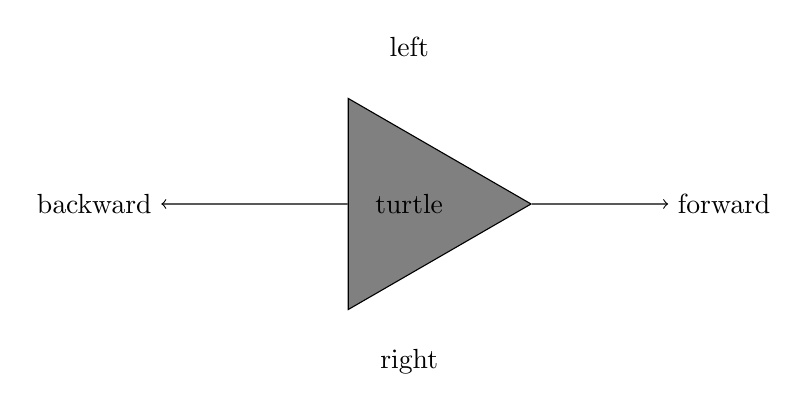
\begin{tikzpicture}

% nodes
\node (bk) at (4, 2) {backward};
\node[turtle] (tt) at (8, 2) {turtle};
\node (fd) at (12, 2) {forward};
\node (lt) at (8, 4) {left};
\node (rt) at (8, 0) {right};

% arrows
\draw[->] (tt) edge (bk);
\draw[->] (tt) edge (fd);

\end{tikzpicture}
\caption{绘图海龟的基本概念}
\end{figure}

Logo 语言的一个关键构造是绘图小海龟,它维持有一个指向,可以前进、后退若干步长,可以左转、右转若干角度。
如果在画布上允许多个海龟的存在,并且每个海龟单独维护自己的步长,所谓的裂解是指如下的变换:

\newpage

\subsection{四阶无限边形镶嵌}

双曲平面上有许多非常有趣的镶嵌结构,这里我们展示一种称为四阶无限边形镶嵌的构造。这个镶嵌结构的构造程序如下

\begin{itemize}
\item 裂解[0, +90, +180, +270; 1]
\item 对所有的小海龟,反复无限次的执行下述命令
\begin{itemize}\item 前进一步 \item 裂解[-90, 0, +90; 1] \end{itemize}
\end{itemize}


\begin{figure}[ht]
\centering
\includegraphics[width=3.5in]{images/H2_tiling_24i-1.png}
\caption{四阶无限边形镶嵌}
\end{figure}

如果注意到双曲平面是一个齐性空间,并且观察到在上述构造里,有些蓝色测地线之间彼此有交点,但这些交点彼此之间没有任何差别;
每一个交点都是两个测地线交汇出来的,都有四支分叉。利用对称性,我们容易理解:

\begin{proposition}
\label{A}
镶嵌结构上的两条测地线如果彼此之间相交,那么它们就是垂直的;否则这两条测地线就是平行的。
\end{proposition}

\begin{proposition}
\label{B}
对于任意一条镶嵌结构上的测地线,镶嵌结构上的其他测地线可以被归类到与之平行或垂直的两组之中。
\end{proposition}

\newpage

\subsection{H-树}

H-树是如下图所示的分形构造。四阶无限边形镶嵌按照一定规则剪枝,拓扑上可以得到H-树。H-树的构造可以非常方便的通过一种支持裂解操作的 Logo 语言来实现。

H-树的具体构造程序如下

\begin{itemize}
\item 对所有的小海龟,反复无限次的执行下述命令
\begin{itemize}\item 前进一步 \item 裂解[-90, +90; $\sqrt{2} / 2$] \end{itemize}
\end{itemize}

\begin{figure}[ht]
\centering
\includegraphics[width=3.5in]{images/2000px-H_tree.png}
\caption{H-树}
\end{figure}

\newpage


\subsection{序数}

\newpage

\section{操作序列与几何}

\subsection{嵌入到镶嵌结构}

给定镶嵌结构上的一条测地线和一个零点,根据 \ref{B} 的结果,我们称与之平行的所有镶嵌结构上的测地线是加性的,
而与之垂直的所有镶嵌结构上的测地线是乘性的。

接着,我们把操作嵌入进来:赋予加性测地线上两个相邻交点之间的连线的含义为操作 i;赋予乘性测地线上两个相邻交点之间的连线的含义为操作 d。

\begin{proposition}
\label{C}
所有可能的操作序列都被嵌入到镶嵌结构上。
\end{proposition}

\begin{proposition}
\label{D}
从规定的零点开始,所有镶嵌结构上的路径,都是合法的操作序列。
\end{proposition}


\subsection{希尔伯特曲线}

\section{一种新的Surreal数?}

\end{document}
